\chapter{Human Audit and Transition Results}
\label{chap:human-results}

This chapter reports the controlling evidence for the final coordination boundary in Debate and Sequential. The audit contains 160 distinct item-configurations drawn from 160 distinct benchmark question identifiers: 80 Debate runs and 80 Sequential runs. These item-configurations produce 400 non-repeat stage records, and 20 blinded duplicate records are inserted only to measure intra-rater repeatability. The item-level dataset contains 15 named fields of mixed type; these are not 15 independent binary error labels.

\section{Human audit reliability}

The 20 hidden repeated stages produced exact agreement of 20/20 on both Discovery and Endorsement, with $\kappa=1.000$ and bootstrap intervals $[1.000,1.000]$. This shows perfect repeatability for the inserted records. It does not show independent inter-annotator validity because the same annotator labelled both blind copies.

Against the frozen Mistral stage labels, human agreement is 330/400 (82.5\%) for Discovery and 322/400 (80.5\%) for Endorsement. Cohen's kappa is 0.632 (95\% bootstrap CI $[0.557,0.705]$) for Discovery and 0.617 ($[0.541,0.691]$) for Endorsement. These values support use of Mistral for broad screening and sampling, but the 70 Discovery disagreements and 78 Endorsement disagreements are not negligible in a transition analysis.

\begin{table}[htbp]
  \centering
  \caption[Human audit reliability]{Human audit reliability. Human--machine agreement uses 400 non-repeat stage records; repeat agreement uses 20 hidden pairs.}
  \label{tab:agreement}
  \begin{tabular}{@{}llrrl@{}}
    \toprule
    Comparison & Axis & Exact agreement & $\kappa$ & 95\% CI \\
    \midrule
    Hidden repeat & Discovery & 20/20 (100.0\%) & 1.000 & [1.000, 1.000] \\
    Hidden repeat & Endorsement & 20/20 (100.0\%) & 1.000 & [1.000, 1.000] \\
    Human--Mistral & Discovery & 330/400 (82.5\%) & 0.632 & [0.557, 0.705] \\
    Human--Mistral & Endorsement & 322/400 (80.5\%) & 0.617 & [0.541, 0.691] \\
    \bottomrule
  \end{tabular}
\end{table}

Across all 420 annotation rows, the 14 cases with Discovery \correct{} and Endorsement \wrong{} demonstrate why a single semantic-correctness label is insufficient. The stage contains the answer but does not support the system selecting it. A presence-oriented judge is likely to over-credit precisely these cases.

\section{Human transition estimates}

The raw audited item transitions differ sharply by architecture. Debate contains 35 \correct$\rightarrow$\correct, 19 \ctow, zero \wtoc, 25 \wrong$\rightarrow$\wrong, and one \uncertain$\rightarrow$\wrong item. Sequential contains 40 \correct$\rightarrow$\correct, four \ctow, six \wtoc, 29 \wrong$\rightarrow$\wrong, and one \uncertain$\rightarrow$\wrong item. Because rare machine-defined transition strata were oversampled, the weighted rates rather than these raw proportions are used for population interpretation.

\begin{figure}[htbp]
  \centering
  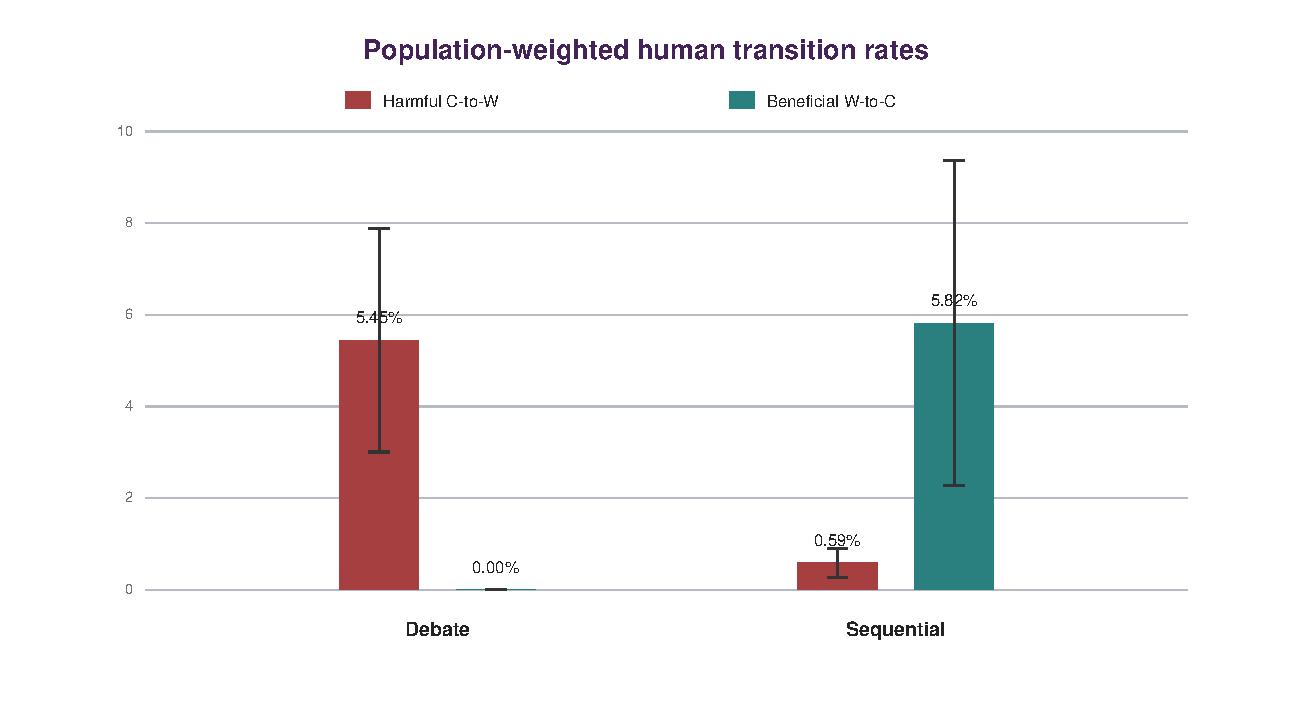
\includegraphics[width=0.88\textwidth]{figures/human_transition_rates.pdf}
  \caption[Population-weighted human transition rates]{Population-weighted human Endorsement transition rates under the primary \uncertain$\rightarrow$\wrong{} rule. Error bars are approximate 95\% finite-population stratified intervals.}
  \label{fig:human-transitions}
\end{figure}

Debate's weighted harmful \ctow{} rate is 5.45\% (approximate 95\% CI $[3.01,7.89]$), compared with 0.59\% for Sequential ($[0.27,0.90]$). The Debate-minus-Sequential difference is 4.86 percentage points ($[2.41,7.32]$). The beneficial \wtoc{} pattern is reversed: 0.00\% for Debate and 5.82\% for Sequential ($[2.28,9.37]$). The one machine-defined Debate beneficial picker event in the sampling census was human \correct$\rightarrow$\correct after unblinding, so no audited Debate wrong source was corrected by the picker.

Using source Discovery rather than source Endorsement gives a weighted probability that a discovered answer is not endorsed in the final output of 7.06\% for Debate and 3.96\% for Sequential. This second measure captures loss between informational presence and decision, including cases where a correct answer was discovered without being cleanly endorsed at the source.

\section{Sensitivity to uncertain labels}

The uncertain-label sensitivity analysis does not reverse the main harmful-rate ordering. Under \uncertain$\rightarrow$\wrong, exclusion of uncertain-bearing items, and \uncertain$\rightarrow$\correct, Debate's harmful rate is 5.45\%, 5.51\%, and 6.58\%, while Sequential's is 0.59\%, 0.60\%, and 2.20\%. The absolute Sequential estimate is more sensitive because one uncertain case has greater influence in a low-rate architecture, but Debate remains higher under every rule.

\section{Scope of the human comparison}

The human transition audit supports a comparison of the final coordination boundaries in Debate and Sequential; it does not by itself explain why SAS outperforms a MAS in a particular benchmark condition. SAS remains part of the final-performance benchmark in \Cref{chap:benchmark-results}. A cross-architecture process comparison should apply the same machine-screening pipeline to SAS and use pre-final Discovery to final Endorsement as the common transition, because SAS has no equivalent multi-agent picker or aggregator. Unless that additional analysis is completed and reported, the dissertation should not claim that SAS wins because it experiences a lower human-audited transition rate.

\section{Chapter summary}

The human audit changes the scale of the machine-screened transition estimates but retains an architecture-specific asymmetry. The final Debate picker is a measurable loss point, whereas the Sequential aggregator is less often destructive and sometimes corrective. This conclusion is bounded to the audited source definitions and weighted sampling frames. It does not establish that Sequential is globally superior to Debate or that the same rates apply to the three other MAS architectures.
